\documentclass[aspectratio=169]{beamer}

\usepackage[brazil]{babel}
\usepackage[utf8]{inputenc}
\usepackage[T1]{fontenc}

\usetheme{Madrid}

\setbeamertemplate{navigation symbols}{}

\title[Apresentação Pessoal]{Apresentação Pessoal}

\author[Diego S. C. Nascimento]{Diego Silveira Costa Nascimento}

\institute[IFRN]{
	Instituto Federal de Educação, Ciências e Tecnologia do Rio Grande do Norte\\
	diego.nascimento@ifrn.edu.br
}

\date[Apresentação]{\today}

\begin{document}

\begin{frame}[plain]
	\includegraphics[scale=0.2]{imagens/IFRN}
	\titlepage
\end{frame}

\logo{\includegraphics[scale=0.1]{imagens/IFRN}}

\begin{frame}
	\frametitle{Sumário}
  	\tableofcontents
\end{frame}

\AtBeginSection[]{
	\begin{frame}
		\frametitle{Sumário}
		\tableofcontents[currentsection]
	\end{frame}
}

\section{Introdução}

\begin{frame}
	\frametitle{De Onde Venho?}

	\begin{block}{Maceió - AL}
		\begin{center}
			\includegraphics[scale=0.4]{imagens/maceio}
		\end{center}
	\end{block}
\end{frame}

\begin{frame}
	\frametitle{Por Que Escolhi a Área de Informática?}

	\begin{itemize}
		\item Admiração pelas ciências exatas;
		\item Curiosidade pela Informática;
		\item Ainda adolescente realizei alguns cursos técnicos:
		\begin{itemize}
			\item Introdução à Informática;
			\item Produção Gráfica;
			\item Manutenção de Computadores; e
			\item Administração de Redes.
		\end{itemize}
	\end{itemize}
\end{frame}

\section{Formação}

\begin{frame}
	\frametitle{Formação Acadêmica}

	\begin{itemize}
		\item Bacharel em Informática -- Análise de Sistemas -- Administração;\\
		\includegraphics[scale=0.1]{imagens/CESMAC-Logo}
		
		\item Licenciado em Informa\c cão e Comunica\c cão;\\
		\includegraphics[scale=0.1]{imagens/IFRN}
		
		\item Especialista em Tecnologia da Informação;\\
		\includegraphics[scale=0.1]{imagens/UFC_Logo}
		
		\item Mestre em Informática Aplicada;\\
		\includegraphics[scale=0.5]{imagens/UNIFOR-Logo}
		
		\item Doutor em Ciências da Computação; e\\
		\includegraphics[scale=0.15]{imagens/ufrn-logo}
		
		\item Pós-doutor em Ciências da Computação.\\
		\includegraphics[scale=0.15]{imagens/ufrn-logo}
	\end{itemize}
\end{frame}

\begin{frame}
	\frametitle{Certifica\c cões}

	\begin{itemize}
		\item Sun Certified Java Programmer;\\
		
\includegraphics[scale=0.2]{imagens/sun}
		
		\item Implantação Cerne de Gestão de Incubadoras;\\
		
\includegraphics[scale=0.2]{imagens/anprotec}
		
		\item Team Kanban Practitioner; e\\
		
\includegraphics[scale=0.2]{imagens/kanban}
	\end{itemize}
\end{frame}


\section{Atuação Profissional}

\begin{frame}
	\frametitle{Atuação Profissional Técnica}

	\begin{itemize}
		\item \textit{Smile} Saúde:
		\begin{itemize}
			\item Função: Digitador;
			\item Tecnologias: \textit{Access} e \textit{Delphi};
		\end{itemize}
		
		\item Cooperativa de Crédito Juriscred:
		\begin{itemize}
			\item Função: Técnico em Informática;
			\item Tecnologias: \textit{Access, Delphi, HTML, PHP, ASP, Windows NT, Linux} e \textit{Clipper/DBU};
		\end{itemize}
		
		\item OFM -- Tecnologia e Informação:
		\begin{itemize}
			\item Função: Programador;
			\item Tecnologias: \textit{Java, JSP/Servlet, OJB, Jasper Report, Oracle} e \textit{Forms/Reports};
		\end{itemize}
		
		\item TecSist:
		\begin{itemize}
			\item Função: Programador;
			\item Tecnologias: \textit{Java, JSP/Servlet, Jasper Report, MySQL, J2ME} e \textit{Linux};
		\end{itemize}
	\end{itemize}
\end{frame}

\begin{frame}
	\frametitle{Atuação Profissional Técnica}
		
	\begin{itemize}
		\item Oboé Financeira:
		\begin{itemize}
			\item Função: Programador;
			\item Tecnologias: \textit{Java, JSP/Servlet, Jasper Report, Oracle, Hibernate} e \textit{Linux};
		\end{itemize}
		
		\item Tergus:
		\begin{itemize}
			\item Função: Programador;
			\item Tecnologias: \textit{Java, JSP/Servlet, Jasper Report, MS SQL Server, Struts} e \textit{Hibernate};
		\end{itemize}
		
		\item Politec:
		\begin{itemize}
			\item Função: Analista de Sistemas;
			\item Tecnologias: \textit{Java, JSP/Servlet, Jasper Report, Struts, JSF, Flex, Hibernate, Oracle, UML, RUP} e Ponto de Função;
		\end{itemize}
	\end{itemize}
\end{frame}

\begin{frame}
	\frametitle{Atuação Profissional Acadêmcia}

	\begin{itemize}
		\item Faculdade de Tecnologia de Alagoas (FAT);
		\item Faculdade da Cidade de Maceió (FACIMA); e
		\item Instituto Federal do Rio Grande do Norte (IFRN).
	\end{itemize}
\end{frame}

\section{Plano de Trabalho}

\begin{frame}
	\frametitle{Projetos de Atuação Profissional}
	
	\begin{itemize}
		\item Oferecer ensino de qualidade;
		\item Fazer parcerias com outras instituições;
		\item Colaborar para o desenvolvimento da região; e
		\item Promover pesquisa e extensão.
	\end{itemize}
\end{frame}

\begin{frame}
	\frametitle{Áreas de Interesse}
	
	\begin{itemize}
        		\item Linguagens de Programação;
		\item Inteligência Artificial; e
		\item Informática na educa\c cão.
	\end{itemize}
\end{frame}

\begin{frame}
	\frametitle{Metodologias de Trabalho}
	
	\begin{itemize}
		\item Aulas expositivas com slides;
		\item Práticas em laboratório;
		\item Lista de exercícios;
	    	\item Prova e 
		\item Projetos prático.
	\end{itemize}
\end{frame}

\begin{frame}
	\frametitle{Wiki Profissional}
	
	\begin{block}{Endereço Eletrônico}
	http://www.diegoscnascimento.wikidot.com/
	\end{block} \vfill
	
	\begin{exampleblock}{Página Web}
		\begin{center}
			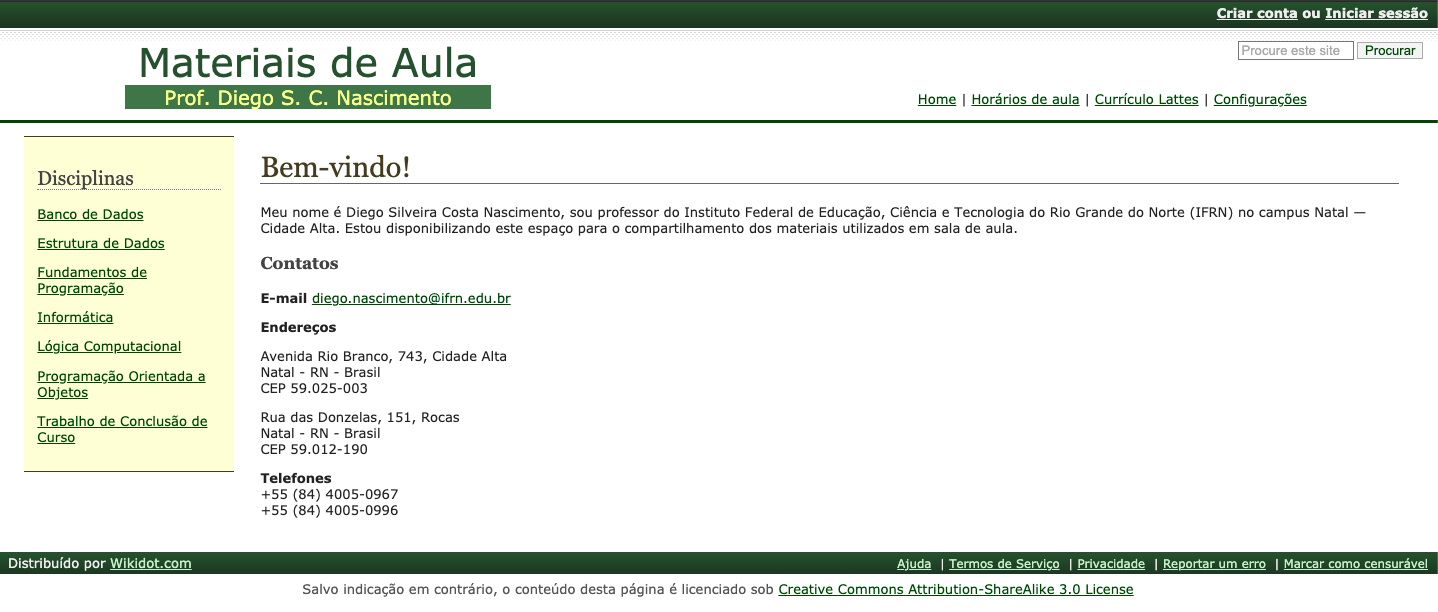
\includegraphics[scale=0.2]{imagens/pagina}
		\end{center}
	\end{exampleblock}
\end{frame}

\section{Conclusão}

\begin{frame}
	\frametitle{Considerações Finais}

	\begin{itemize}
		\item Possuo formação técnica e acadêmica continuada;
		\item Adquiri experiências em várias organizações na área na qual fui
		professor (Sistemas de Informação);
		\item Tenho atuação em pesquisa de ponta; e
		\item Estou motivado e comprometido em colaborar para capacitação
		profissional, bem como, para o desenvolvimento nacional, seja ele industrial ou científico.
	\end{itemize}
\end{frame}

\end{document}